% !TEX root = ../main.tex


\section{Run To Completion}
\label{sec:run-completion}
The run to completion semantics is specified via an abstract basis that is extended by the model~\cite{MoSnHo18,MoSnHo-ABZ2020}. 
Figure~\ref{fig:basis} shows a state-chart representation of how the basis enforces 
the run to completion semantics on the model transitions. 

\ColinInlineComment{the Fig.1 needs updating wrt to queues.. e.g. eQ and iQ should be content(eQ) and content(iQ).
	also NoTriggeredTransitionsEnable should be NoTriggeredTransitionsEnabled}
\begin{figure}[!h]
	\vspace{-.4cm}
	\centering
	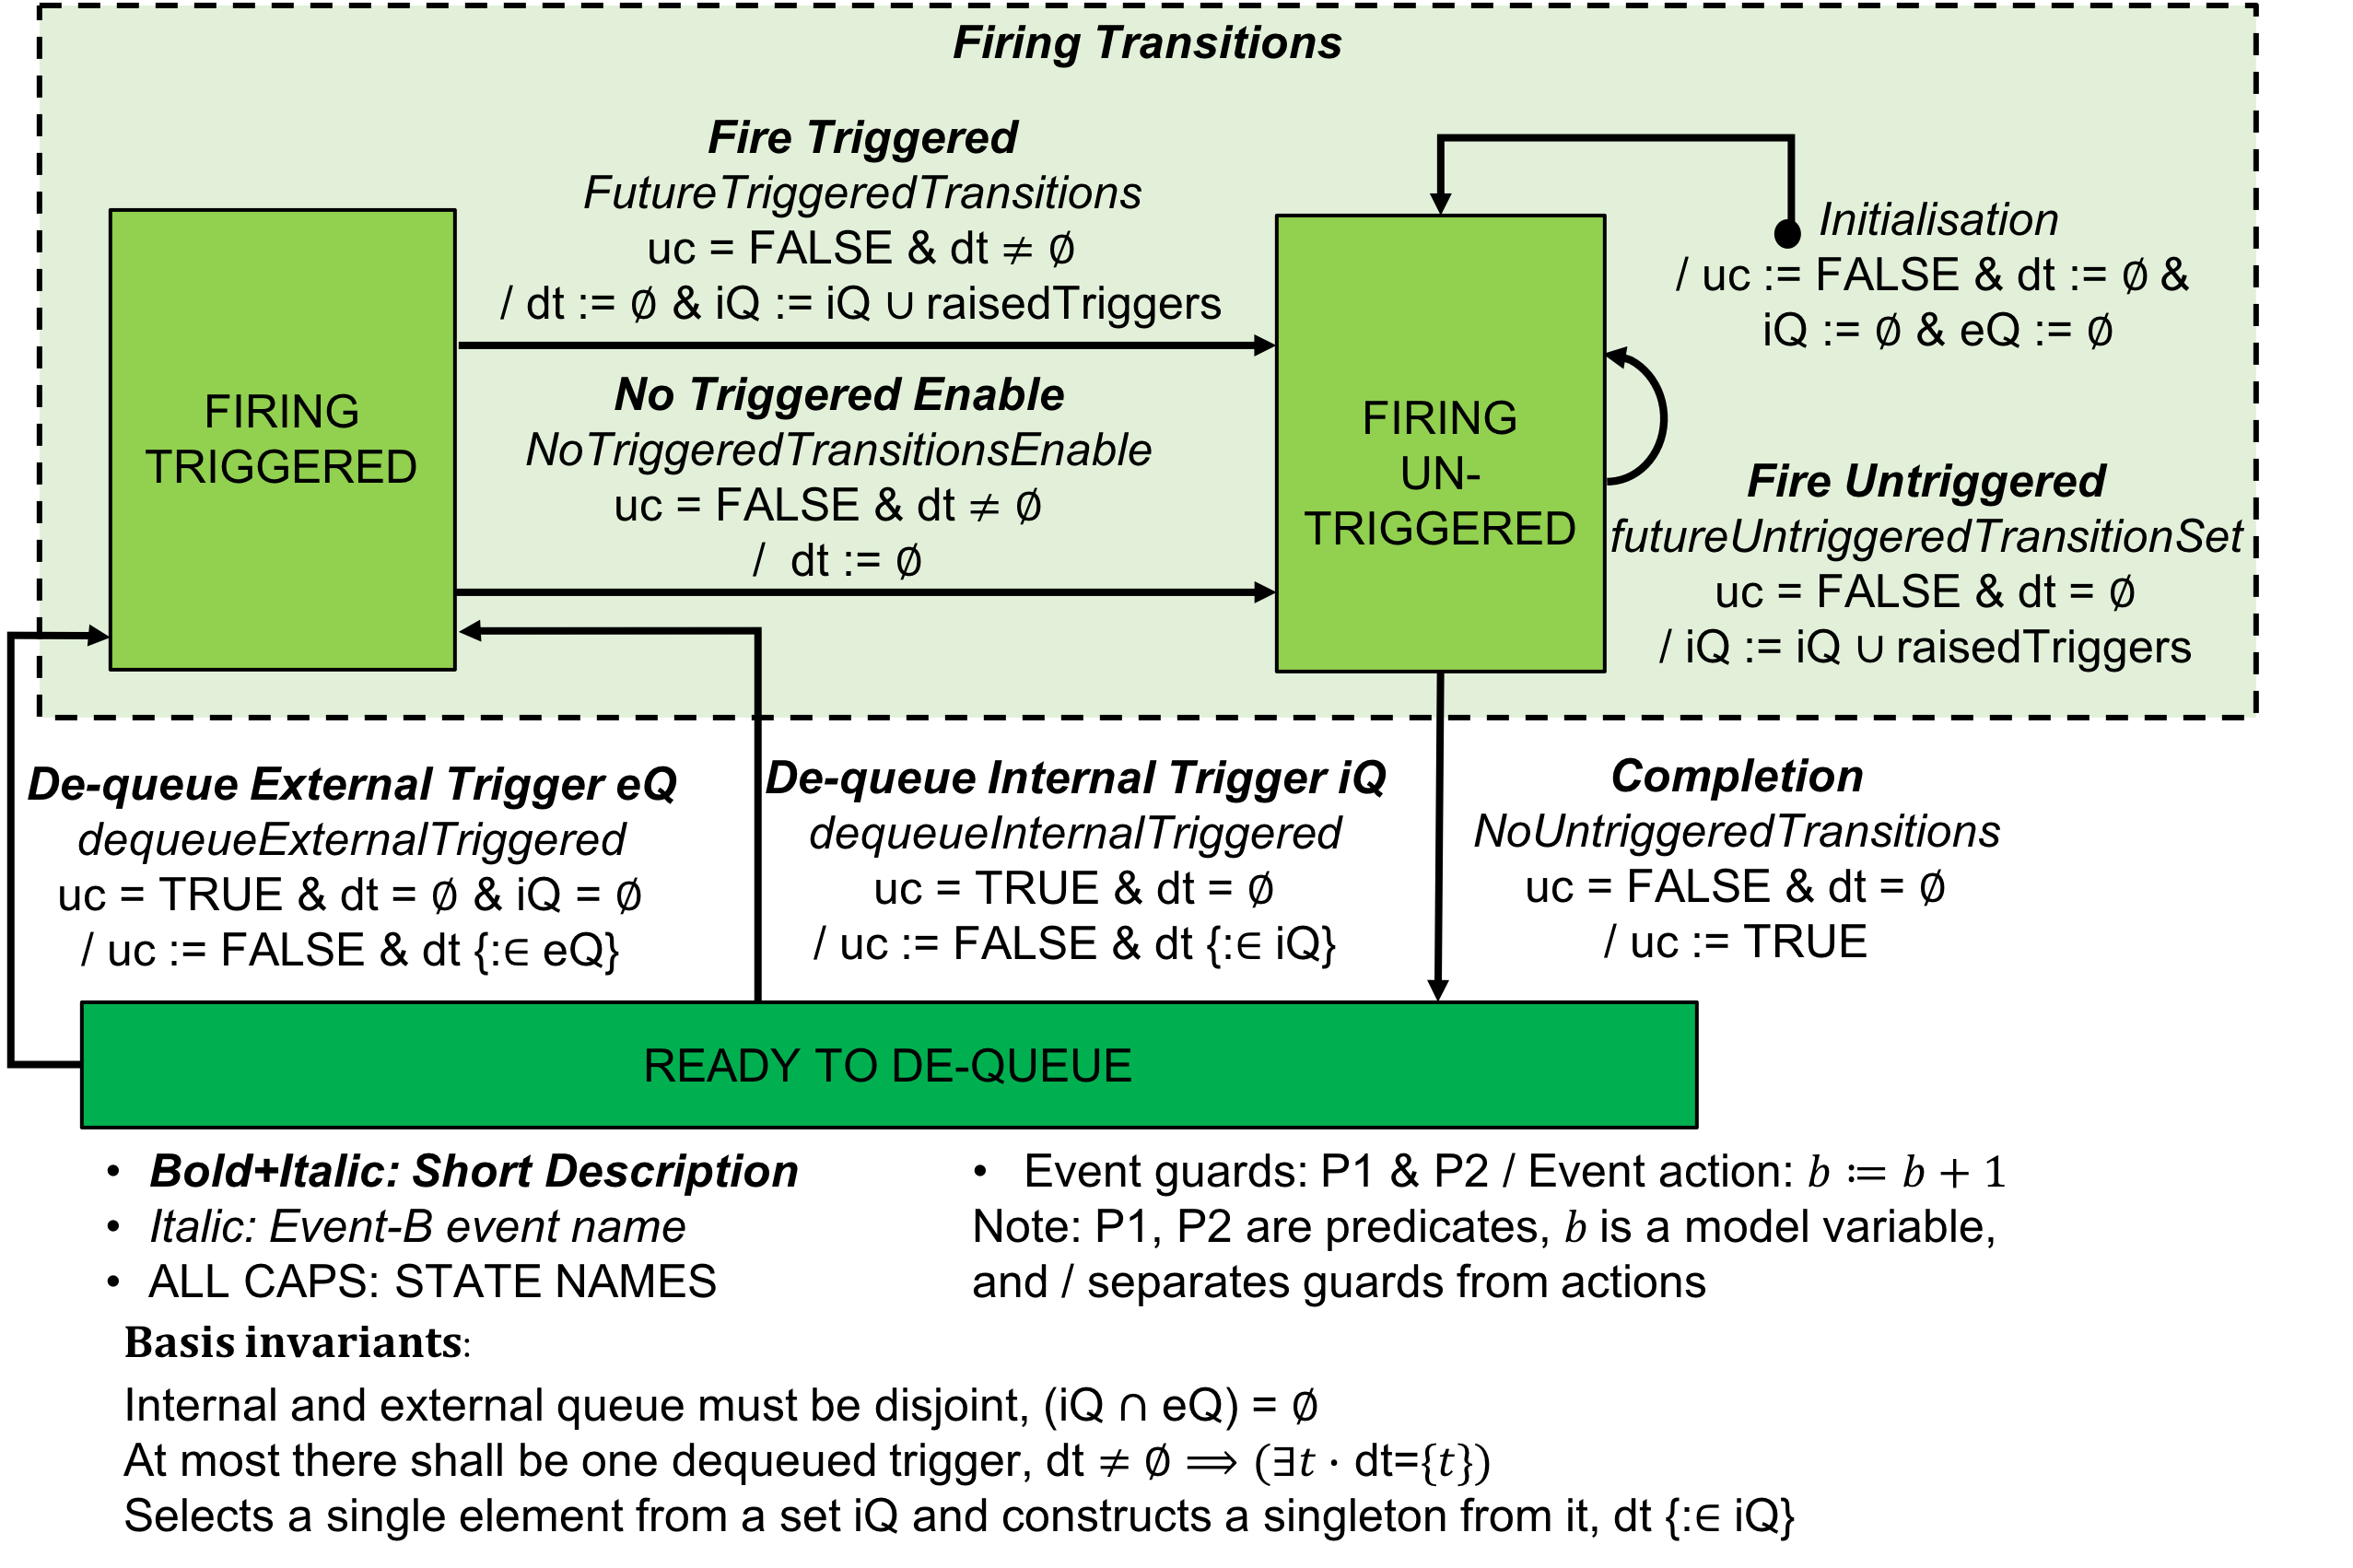
\includegraphics[width=0.90\textwidth, trim=30 50 60 0]{figures/Picture6.png}
	\caption{Abstract representation of run to completion basis}
	\label{fig:basis}
	\vspace{-.4cm}
\end{figure}

The specification of this basis consists of an \EVENTB \emph{context} and \emph{machine} that are the same for all input models and are refined by the specific output of the translation.  
The basis context, shown in listing \ref{lst:BasisContext}, introduces a set of all possible triggers, |SCXML_TRIGGER| which is partitioned into internal and external triggers 
(e.g |FutureInternalTrigger| and |FutureExternalTrigger| respectively), 
some of which will be introduced in future refinements. 
At each refinement these trigger sets are further partitioned to introduce more concrete triggers, 
leaving a new abstract set to represent the remaining triggers yet to be introduced. 

The context also models \emph{sequences} of triggers as a data type to be used for the trigger queues.
Our initial work modelled queues abstractly as sets of triggers which was adequate for most verification purposes but does not enforce fairness on trigger consumption. 
Hence we were forced to introduce fairness assumptions regarding trigger consumption in order to verify liveness properties.
In this paper we introduce sequences to properly model the trigger queues which are an implementation of this fairness property. 
Note that the queue also enables the same trigger to be raised twice in the queue which was not possible in a set.
The constant |Seq| returns the set of all possible sequences of a given subset of triggers and is defined using lambda calculus.
Constant functions are also defined for the usual operations on sequences: 
\emph{length} of a given sequence, 
\emph{append} a trigger to the end of a sequence to give a new sequence, 
\emph{concat}enate two sequences to give a new sequence, 
return the trigger at the \emph{head} of a sequence, 
return the sequence that makes up the \emph{tail} of a sequence and 
return the \emph{content} (set of triggers) involved in a sequence. 
The Basis context also defines several theorem properties about sequences that are needed to discharge proof obligations.
These are omitted from Listing~\ref{lst:BasisContext} for brevity.

\ColinInlineComment{I changed the comments to a command in order to get them to align.  Is there a better way? }
\newcommand*{\Comment}[1]{\color{green!50!black}\hfill\makebox[0.6\textwidth][l]{#1}}%

 \begin{lstlisting}[caption={Abstract basis context},label={lst:BasisContext}, language=Event-B, tabsize=8, escapechar=€, frame=single, basicstyle=\rmfamily\scriptsize, belowskip=-2.0 \baselineskip, float=t]
 context
 	basis_c 	€\Comment{// (generated for SCXML)}€
 sets
 	SCXML_TRIGGER	 €\Comment{// all possible triggers}€
 constants
 	FutureInternalTrigger	€\Comment{// all possible internal triggers}€
 	FutureExternalTrigger	€\Comment{// all possible external triggers}€
 	Seq							€\Comment{// return all possible sequences of given set of triggers}€
 	Seq_length					€\Comment{// return the length of a sequence of triggers}€
 	Seq_append					€\Comment{// return the result of appending trigger to a sequence}€
 	Seq_concat					€\Comment{// return the concatenation of two sequences of triggers}€
 	Seq_head					€\Comment{// return the trigger at head of a sequence of triggers}€
 	Seq_tail					€\Comment{// return the sequence at tail of a sequence of triggers}€
 	Seq_content					€\Comment{// return the set of triggers in a sequence of triggers}€
 	InternalQueueType			€\Comment{// type of internal queues}€
 	ExternalQueueType			€\Comment{// type of external queues}€
 	
 axioms
 	partition(SCXML_TRIGGER, FutureInternalTrigger, FutureExternalTrigger) 
 	Seq = (λT · T ⊆ SCXML_TRIGGER ∣ {n, s · n ∈ ℕ ∧ s ∈ 0 ‥ n − 1 → T ∣ s})
 	Seq_length = (λs · s ∈ Seq(SCXML_TRIGGER) ∣ card(s))
 	Seq_append = (λ s ↦ t · s ∈ Seq(SCXML_TRIGGER) ∧ t ∈ SCXML_TRIGGER ∣ 
 		{i↦v ∣ i ∈ 0 ‥ Seq_length(s) ∧ (i < Seq_length(s) ⇒ v = s(i)) ∧ (i = Seq_length(s) ⇒ v = t) } )
	Seq_concat = (λ s1 ↦ s2 · s1 ∈ Seq(SCXML_TRIGGER) ∧ s2 ∈ Seq(SCXML_TRIGGER) ∣ 
		{i↦v ∣ i ∈ 0 ‥ Seq_length(s1) + Seq_length(s2) − 1 ∧ (i < Seq_length(s1) ⇒ 
									v = s1(i)) ∧ (i ≥ Seq_length(s1) ⇒ v = s2(i − Seq_length(s1))) } )
	Seq_head = (λs · s ∈ Seq(SCXML_TRIGGER) ∧ s ≠ ∅ ∣ s(0))								
	Seq_tail = (λs· s∈Seq(SCXML_TRIGGER) ∧ s≠∅ ∣ {i↦v ∣ i∈0‥Seq_length(s)−2 ∧ v=s(i+1)} )	
	Seq_content = (λs · s ∈ Seq(SCXML_TRIGGER) ∣ ran(s))
	InternalQueueType = Seq(FutureInternalTrigger)
	ExternalQueueType = Seq(FutureExternalTrigger)
 end
 \end{lstlisting}	

Each of the transitions in the basis (see Figure~\ref{fig:basis}) represents an abstract event of the basis machine (Listing~\ref{lst:BasisMachine}) that describes the generic behaviour of models under a run to completion semantics.
These events provide an abstraction that defines the altering of trigger queues and completion flag. 
\EventB refinement rules prohibit new events from modifying abstract variables (i.e. new events refine `skip').
Hence, since \SCXML transitions need to modify the trigger queues etc., used to capture the \SCXML run to completion semantics, all events generated by translation of the specific \SCXML model,  must refine abstract events introduced for this purpose in the basis.
The basis machine also declares variables that correspond to the currently dequeued trigger,  |dt|, 
the queue of internal triggers raised by actions within the model, |iQ|, 
the queue of external triggers raised by the environment, |eQ|,
and a flag, |uc|, that signals when a run to completion macro-step has been completed 
(no un-triggered transitions are enabled). 
Note that, for convenience, the currently dequeued trigger is modelled as a singleton set which may be empty (i.e. consumed) or contain the single trigger to be consumed.

The trigger queues and dequeued trigger are initialised to empty and |uc| is set to |FALSE| so that any enabled un-triggered transitions are dealt with via the |futureUntriggeredTransitionSet| event when the system first starts (see Listing~\ref{lst:scxml-r2c}).
This will subsequently enable completion and reset the |uc| flag to |TRUE|.
The abstract event |futureRaiseExternalTrigger| represents the raising  of an external trigger (not shown in the diagram).    
After completion, a queued trigger can be prepared for consumption by moving it to the dequeued trigger, |dt|.
Internal triggers have a higher priority, since the external trigger queue is only dequeued if the |iQ| is empty (see |dequeueExternalTriggered| and |dequeueInternalTriggered| in Figure~\ref{fig:basis}).
The abstract event |futureTriggeredTransitionSet| represents a combination of parallel transitions that may be simultaneously triggered by the dequeued trigger, |dt|.
When the actual example \SCXML is translated, a separate refinement of this abstract event will be generated for each subset of the set of parallel transitions that could fire in parallel in order to cater for all possibilities of enablement, however, as the model is refined some combinations may be eliminated as the guards are strengthened.
This approach to generating an event for each possible combination of each set of transitions that could fire in parallel is needed because of the batch enabling semantics of the SCXML run to completion (see Section~\ref{sec:scxml}).
The actions of these transitions may also raise triggers of their own in the internal trigger queue |iQ|.


Completion of triggered and untriggered transitions may be non-deterministically premature to allow future refinements to strengthen the guards of transitions (i.e. to disable them resulting in an earlier completion).
In the process of refining a model, a designer takes advantage of this non-determinism in the abstraction by adding nested sub-states and explicit guards to transitions. 
When a refinement level is reached where the designer wants to enforce a requirement (i.e. prevent it being bypassed by a non-deterministic completion), the model needs to be \emph{finalised} (see Section~\ref{sec:translation} for more on finalisation). 
The \SCXML translation tool will then automatically strengthen the guards of events |noTriggeredTransitionsEnabled| and |noUntriggeredTransitionsEnabled|, to ensure that the run to completion sequence is not interrupted by non-deterministic behaviour. 
To do this we need to guard completion so that it cannot happen while any relevant transition is still enabled.
To finalise a triggered transition, the guard of |noTriggeredTransitionsEnabled| is strengthened by adding the conjunction of the negated guards of all transitions that can fire in parallel with the transition being finalised.
%(To fire in parallel a transition must be in a parallel region of the state-chart and be triggered by the same trigger).
Similarly, to finalise an untriggered transition, the guard of |noUntriggeredTransitionsEnabled| is strengthened by adding the conjunction of the negated guards of all untriggered transitions that can fire in parallel.
It may seem that finalisation could cause an unmanageable explosion of guards.
However, to fire in parallel, transitions must be contained in parallel regions and also be enabled by the same trigger (or be un-triggered).
In practice, since most systems do not contain many parallel regions, the number of transitions that can fire in parallel is limited.
Transition finalisation can be left until it is needed for the proof of a particular property and does not generate any new proof obligations since adding guards is a trivial refinement step.
Finalisation is also needed in order to remove non-deterministic behaviours when the model is animated for validation purposes.

% The basis machine declares variables 
% that correspond to the triggers present in the queue at any given time, and a flag, |SCXML_uc|, that signals when a run to completion macro-step has been completed (no un-triggered transitions are enabled). 
% After initialisation, both trigger queues are empty and |SCXML_uc| is set to |FALSE| so that un-triggered transitions are dealt with. 
% The basis machine provides events that describe the generic behavior of models that follow the run to completion semantics in terms of altering the trigger queues and completion flag.
% Since new events introduced in a refinement cannot modify existing variables, all future events generated by translation of the specific \SCXML model, will refine these abstract events.
% The abstract event, |SCXML_futureRaiseExternalTrigger| represents the raising of an external trigger (this transition is not shown in the diagram).    
% The abstract event, |SCXML_futureInternalTransitionSet| represents a combination of transitions that are triggered by an internal trigger. 


% The guards of this event ensure prior completion of the previous macro-step. 
% A similar event, |SCXML_futureExternalTransitionSet| (not shown) represents a combination of transitions that are triggered by an external trigger and has the additional guard that the internal trigger queue is empty.
% These two triggered transition events reset the completion flag to ensure that any un-triggered transitions that may have become enabled have a chance to fire next.
% The abstract event |SCXML_futureUntriggeredTransitionSet| represents a combination of transitions that are un-triggered and may only be fired when the completion flag is unset (FALSE).
% It leaves the completion flag unset in case further combinations of un-triggered transitions are enabled.
% All three of these transition events also allow for raising a non-deterministic set of internal triggers.
% A final abstract event, |SCXML_completion|, sets the completion flag (TRUE) if it is not already set. At this abstract basis level, this is non-deterministically fired since we do not yet have any detail of what needs to be completed.




 \begin{lstfloat}[!tb]
 \begin{lstlisting}[caption={Abstract basis machine}, label={lst:BasisMachine},language=Event-B, escapechar=€, frame=single, basicstyle=\rmfamily\scriptsize, belowskip=-2.0 \baselineskip]
 MACHINE	basis	   €\Comment{//   (generated for SCXML)}€
 SEES    	basis_ctx
 VARIABLES
 €~~€	iQ	   €\Comment{//   internal trigger queue}€
 €~~€	eQ	   €\Comment{//   external trigger queue}€
 €~~€	uc	   €\Comment{//   run to completion flag}€
 €~~€	dt	   €\Comment{//   dequeued trigger for this run}€
 INVARIANTS
 €~~€	iQ ∈ InternalQueueType	   	€\Comment{//   internal queue}€
 €~~€	eQ ∈ ExternalQueueType	   	€\Comment{//   external queue}€
 €~~€	uc ∈ BOOL	   				€\Comment{//   completion flag}€
 €~~€	dt ⊆ SCXML_TRIGGER	   		€\Comment{//   dequeued trigger}€
 €~~€	dt≠∅ ⇒(∃t·dt={t})			€\Comment{//   at most one dequeued trigger}€
 EVENTS
 	INITIALISATION   €\Comment{// queues empty, completion false, no dequeued triggers}€
 			iQ, eQ, uc, dt ≔ ∅,	∅, FALSE, ∅  
 	END

 	futureRaiseExternalTrigger      	   €\Comment{//basis of future event to raise an external trigger}€
 		ANY 	raisedTrigger	WHERE raisedTrigger ∈ FutureExternalTrigger
 		THEN	eQ≔append(eQ ↦ raisedTrigger)
 	END

 	dequeueInternalTrigger      	   €\Comment{//event to dequeue an internal trigger}€ 
 		WHEN	iQ≠∅ & dt=∅ & uc=TRUE 
 		THEN	dt, iQ, uc ≔ {head(iQ)}, tail(iQ), FALSE
 	END

 	dequeueExternalTrigger      	   €\Comment{//event to dequeue an external trigger}€ 
 		WHEN	eQ≠∅ & dt=∅ & uc=TRUE & iqQ∅
		THEN	dt, eQ, uc ≔ {head(eQ)}, tail(eQ), FALSE
 	END

 	futureTriggeredTransitionSet      	€\Comment{//basis of future event representing triggered transitions}€
 		ANY trigger, raisedTriggers WHERE trigger ∈ dt & uc = FALSE & raisedTriggers ∈ Seq(FutureInternalTrigger)
 		THEN	dt, iQ ≔ ∅ , concat(iQ↦raisedTriggers)
 	END

 	noTriggeredTransitionsEnabled      	€\Comment{//event to fire when no triggered transitions enabled}€ 
 		WHEN 	uc=FALSE & dt≠∅
 		THEN	dt ≔ ∅
 	END

 	futureUntriggeredTransitionSet      €\Comment{//basis of future event representing untriggered transitions}€
 		ANY	raisedTriggers	WHERE	uc=FALSE & dt=∅ & raisedTriggers∈Seq(FutureInternalTrigger)
 		THEN iQ ≔ concat(iQ↦raisedTriggers)
 	END

 	noUntriggeredTransitionsEnabled      €\Comment{//event fired when no untriggered transitions enabled}€
 		WHEN	uc=FALSE & dt=∅
 		THEN	uc ≔ TRUE
 	END
 END
 \end{lstlisting}
 \end{lstfloat}

% \begin{lstfloat}[!tb]
% \begin{lstlisting}[caption={Event-B event corresponding to internal triggered transition to \textbf{Wait50ms} state in refinement level 1 shown in Fig.~\ref{fig:ASIC}}, label={lst:SecBotMach0},language=Event-B, escapechar=|, frame=single, belowskip=-2.0 \baselineskip]
% spi_done__InitialiseSensor_Wait50ms:	
% refines SCXML_futureInternalTransitionSet 
% any SCXML_it SCXML_raisedTriggers where
% SCXML_it  ∈ SCXML_iq 
% SCXML_uc = TRUE
% SCXML_raisedTriggers ⊆ SCXML_FutureInternalTrigger
% InitialiseSensor = TRUE
% SCXML_it = spi_done  	//trigger for this transition |\label{line:defTrigger}|
% then
% SCXML_uc ≔ FALSE
% SCXML_iq ≔ (SCXML_iq ∪ SCXML_raisedTriggers) ∖ {SCXML_it}
% InitialiseSensor ≔ FALSE
% Wait50ms ≔ TRUE
% end
% \end{lstlisting}
% \end{lstfloat}

%%% Local Variables:
%%% mode: latex
%%% TeX-master: "../main"
%%% End:
